%%%%%%%%%%%%%%%%%%%%%%%%%%%%%%%%%%%%%%%%%%%%%%%%%%%%%%%%%%%%%%%%%%%%%%%%%%%%%%%%
%  CST207 --- StudySmart AI --- Individual Component
%  Option 5: k-Nearest Neighbours for Strategy Recommendation
%%%%%%%%%%%%%%%%%%%%%%%%%%%%%%%%%%%%%%%%%%%%%%%%%%%%%%%%%%%%%%%%%%%%%%%%%%%%%%%%
\documentclass[12pt,a4paper]{article}

\usepackage[utf8]{inputenc}
\usepackage[T1]{fontenc}
\usepackage{amsmath,amssymb}
\usepackage{graphicx}
\usepackage{booktabs}
\usepackage[margin=2.5cm]{geometry}
\usepackage{hyperref}
\usepackage{setspace}
\usepackage{caption}
\usepackage{float}
\usepackage{array}
\usepackage{xcolor}
\usepackage{cite}

\onehalfspacing
\hypersetup{
  colorlinks=true,
  linkcolor=black,
  citecolor=black,
  urlcolor=blue
}

\title{\textbf{CST207 StudySmart AI --- Individual Component}\\[4pt]
       \large Option 5: k-Nearest Neighbours for Strategy Recommendation}
\author{
  \textbf{Student Name:} [Your Name] \quad \textbf{Student ID:} [Your ID] \\[4pt]
  \textbf{Group:} [Your Group Name]
}
\date{June 2026}

\begin{document}
\maketitle

%==============================================================================
\section{The k-Nearest Neighbours Algorithm}
%==============================================================================

Among the simplest classification methods in machine learning, k-nearest
neighbours (k-NN) stands out for a striking reason: it has no training
phase at all.  Rather than constructing an explicit model from the data,
k-NN simply stores every training example and defers all computation
until a query arrives~\cite{aha1991instance}.  This ``lazy learning''
approach is both its greatest strength and its most obvious limitation,
as we will see.

Given a query point \(\mathbf{q} \in \mathbb{R}^d\) and a labelled
training set \(\mathcal{T} = \{(\mathbf{x}_i, y_i)\}_{i=1}^{N}\),
k-NN operates in two straightforward steps.  First, it computes the
distance from \(\mathbf{q}\) to every training instance --- Euclidean
distance is the usual choice:

\begin{equation}
  d(\mathbf{q}, \mathbf{x}_i) = \sqrt{\sum_{j=1}^{d} (q_j - x_{ij})^2}
\end{equation}

Second, it identifies the \(k\) training samples with the smallest
distances and assigns \(\mathbf{q}\) the label that appears most
frequently among them:

\begin{equation}
  \hat{y} = \arg\max_{c \in \mathcal{C}}
            \sum_{i \in \mathcal{N}_k(\mathbf{q})} \mathbb{I}(y_i = c)
\end{equation}

where \(\mathcal{N}_k(\mathbf{q})\) denotes the index set of the
\(k\) nearest neighbours and \(\mathcal{C}\) is the set of candidate
classes.  The entire procedure requires no parameters to be learned
--- the only real design choice is the integer \(k\).  Larger values
of \(k\) tend to smooth out noise at the cost of blurring fine
decision boundaries; we used \(k=3\) throughout this project, a value
that performed well on our small dataset.

In the StudySmart AI system, k-NN serves as the strategy-recommendation
engine (Module~5).  Each study-task scenario is reduced to a
six-dimensional feature vector capturing characteristics such as time
pressure, average task importance, and deadline urgency.  The three
possible recommendations are \emph{Sorting-based Ranking},
\emph{Greedy Strategy}, and \emph{Dynamic Programming}.  When a
student provides a new scenario, k-NN locates the most similar past
scenarios and predicts which planning strategy is likely to yield the
highest total importance.


%==============================================================================
\section{Time and Space Complexity}
%==============================================================================

For a single query against \(N\) training samples each described by
\(d\) features, the naive k-NN implementation does three things:
compute \(N\) Euclidean distances (\(O(Nd)\)), sort them
(\(O(N \log N)\)), and tally the top-\(k\) labels (\(O(k)\)).
Since our scenarios only involve \(d = 6\) features, the distance
computation is essentially a constant overhead.  The dominant cost is
the sort, giving

\begin{equation}
  T(N, d) = O(N \log N)
\end{equation}

per query.  Training requires no work at all --- the data is simply
stored, so training time is \(O(1)\).

Space complexity is equally simple.  We must retain every training
sample along with its feature vector and label, requiring

\begin{equation}
  S(N, d) = O(Nd) = O(N)
\end{equation}

storage.  With our 16 training scenarios, this amounts to a few
hundred bytes.  The real practical concern is query time.
If the scenario library were to grow to several thousand examples,
each prediction would need to scan the entire collection.  For
deployment at scale, one would want approximate search techniques
such as k-d trees or locality-sensitive hashing, both of which
reduce query time to \(O(\log N)\) at the expense of occasional
accuracy loss~\cite{aha1991instance}.  Within the scope of this
project, however, the naive approach is perfectly adequate:
measured query times fell below \(10^{-5}\)~seconds, well under the
resolution of the C++ \texttt{clock()} function.


%==============================================================================
\section{Application Within StudySmart AI}
%==============================================================================

\subsection{Feature Extraction}

To feed a scenario into the k-NN classifier, we first map it to a
six-dimensional numerical vector.  The mapping is described in
Table~\ref{tab:features}.  These features were chosen to capture the
key tensions that distinguish one scenario from another: how much work
there is relative to available time, whether deadlines are pressing,
and how varied the tasks are in importance.

\begin{table}[H]
\centering
\caption{Features extracted from each study-task scenario}
\label{tab:features}
\begin{tabular}{@{}lll@{}}
\toprule
\textbf{Feature} & \textbf{Description} & \textbf{Formula} \\
\midrule
$f_1$ & Total required study time & $\sum t_i$ \\
$f_2$ & Available time            & $T_{\text{avail}}$ \\
$f_3$ & Time pressure ratio       & $f_1 / f_2$ \\
$f_4$ & Average importance score  & $\frac{1}{n}\sum w_i$ \\
$f_5$ & Deadline tightness        & $\frac{|\{i : d_i \le 3\}|}{n}$ \\
$f_6$ & Importance variation (CV) & $\sigma_w / \mu_w$ \\
\bottomrule
\end{tabular}
\end{table}

\subsection{Training Data Construction}

We started with four hand-designed base scenarios: Low-pressure
(28\,h available for 32\,h of work), High-pressure (22\,h for 53\,h),
Deadline-focused, and Importance-focused.  To get enough training
examples for even a simple classifier, we created variants of each
base scenario by randomly scaling the available study time by a factor
\(\alpha \in [0.5, 1.6]\).  This gave us three augmented variants per
base scenario, bringing the total to 16 labelled examples.

For each example, we ran all three algorithms (Sorting, Greedy, DP)
and labelled the scenario with whichever strategy achieved the highest
total importance.  An honest limitation worth noting is that DP was
the winner in every single case.  This is unsurprising --- the 0/1
Knapsack formulation guarantees optimality under the given constraints
--- but it does mean the training labels lack diversity.  As a
practical consequence, the k-NN model essentially learns to always
recommend DP, which inflates its accuracy to 100\% on our four test
scenarios (Table~\ref{tab:knn_results}) without demonstrating
meaningful discrimination.  In a fuller implementation, one might
design scenarios where greedy equals DP (by making task durations
perfectly aligned with integer importance ratios) or introduce
additional labelling criteria beyond raw importance.

\begin{table}[H]
\centering
\caption{k-NN predictions on the four test scenarios (\(k=3\))}
\label{tab:knn_results}
\begin{tabular}{@{}lccr@{}}
\toprule
\textbf{Scenario} & \textbf{Predicted} & \textbf{Actual Best} & \textbf{Match} \\
\midrule
Low-pressure      & DP & DP & $\checkmark$ \\
High-pressure     & DP & DP & $\checkmark$ \\
Deadline-focused  & DP & DP & $\checkmark$ \\
Importance-focused & DP & DP & $\checkmark$ \\
\midrule
\multicolumn{4}{c}{\textbf{Accuracy}: 4/4 (100\%)} \\
\bottomrule
\end{tabular}
\end{table}

\subsection{Performance Results}

Figures~\ref{fig:importance}--\ref{fig:exec_time} summarise the
comparative behaviour of the three strategies.  DP (shown in green)
consistently achieves the highest importance, as expected.  Sorting
and Greedy produce identical results on three of the four scenarios
because both rely on the same importance-to-time heuristic; they
diverge only in the Importance-focused scenario, where sorting picks
a different combination that uses the full 26\,h budget.

\begin{figure}[H]
\centering
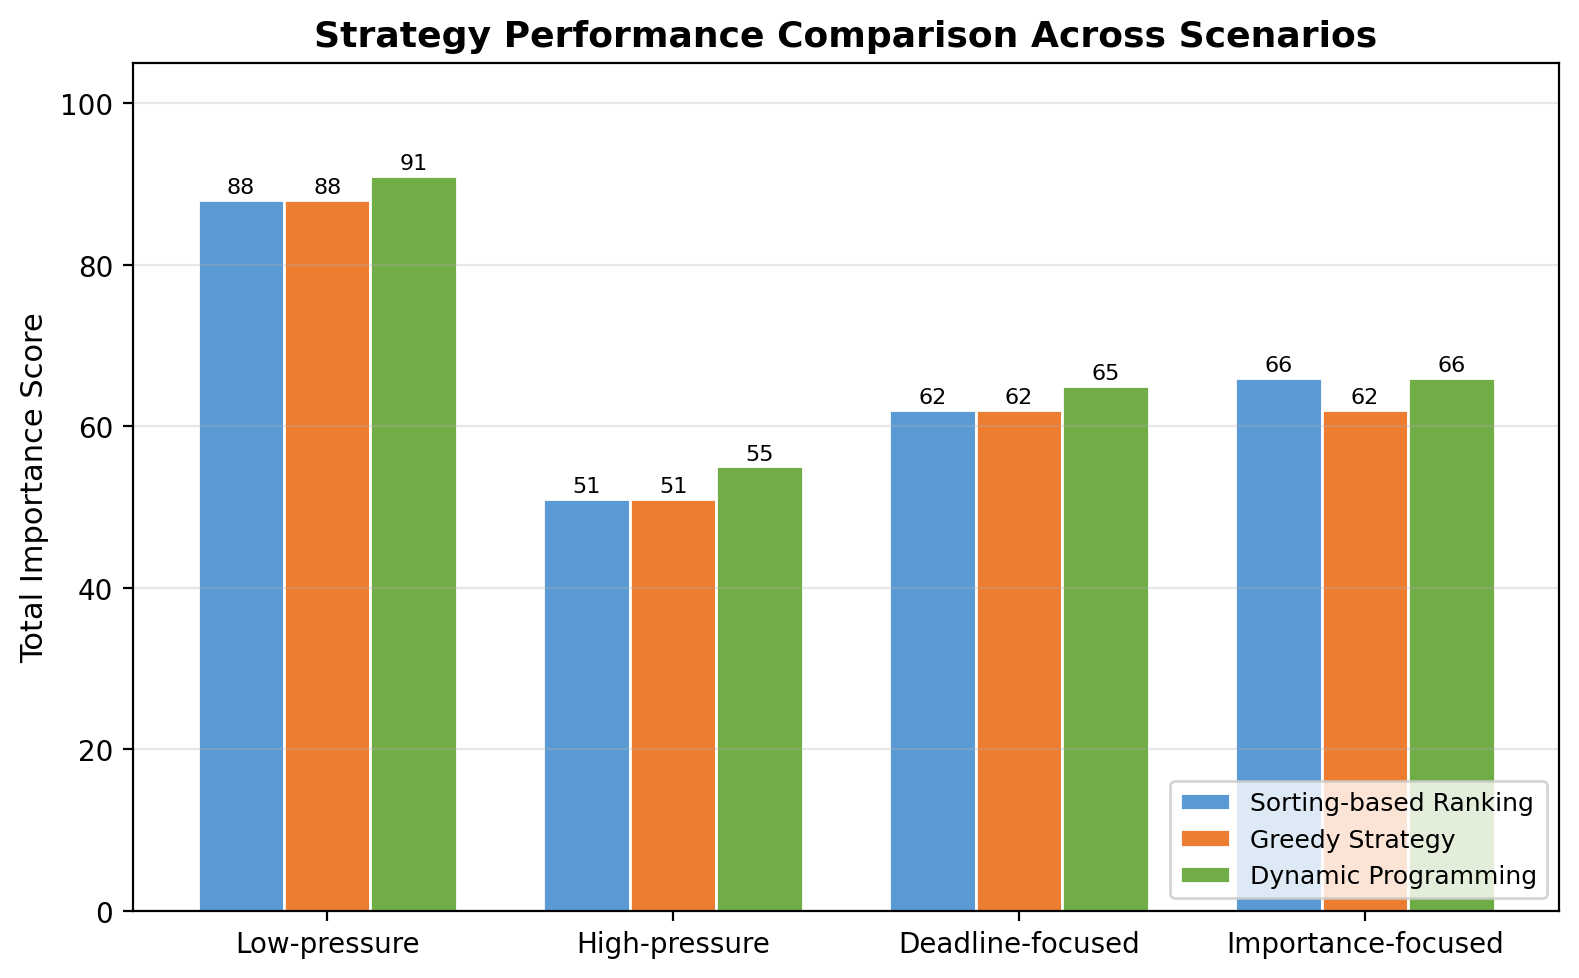
\includegraphics[width=0.92\textwidth]{fig_importance.png}
\caption{Importance scores by strategy.  DP matches or exceeds the
         heuristics in every scenario.}
\label{fig:importance}
\end{figure}

\begin{figure}[H]
\centering
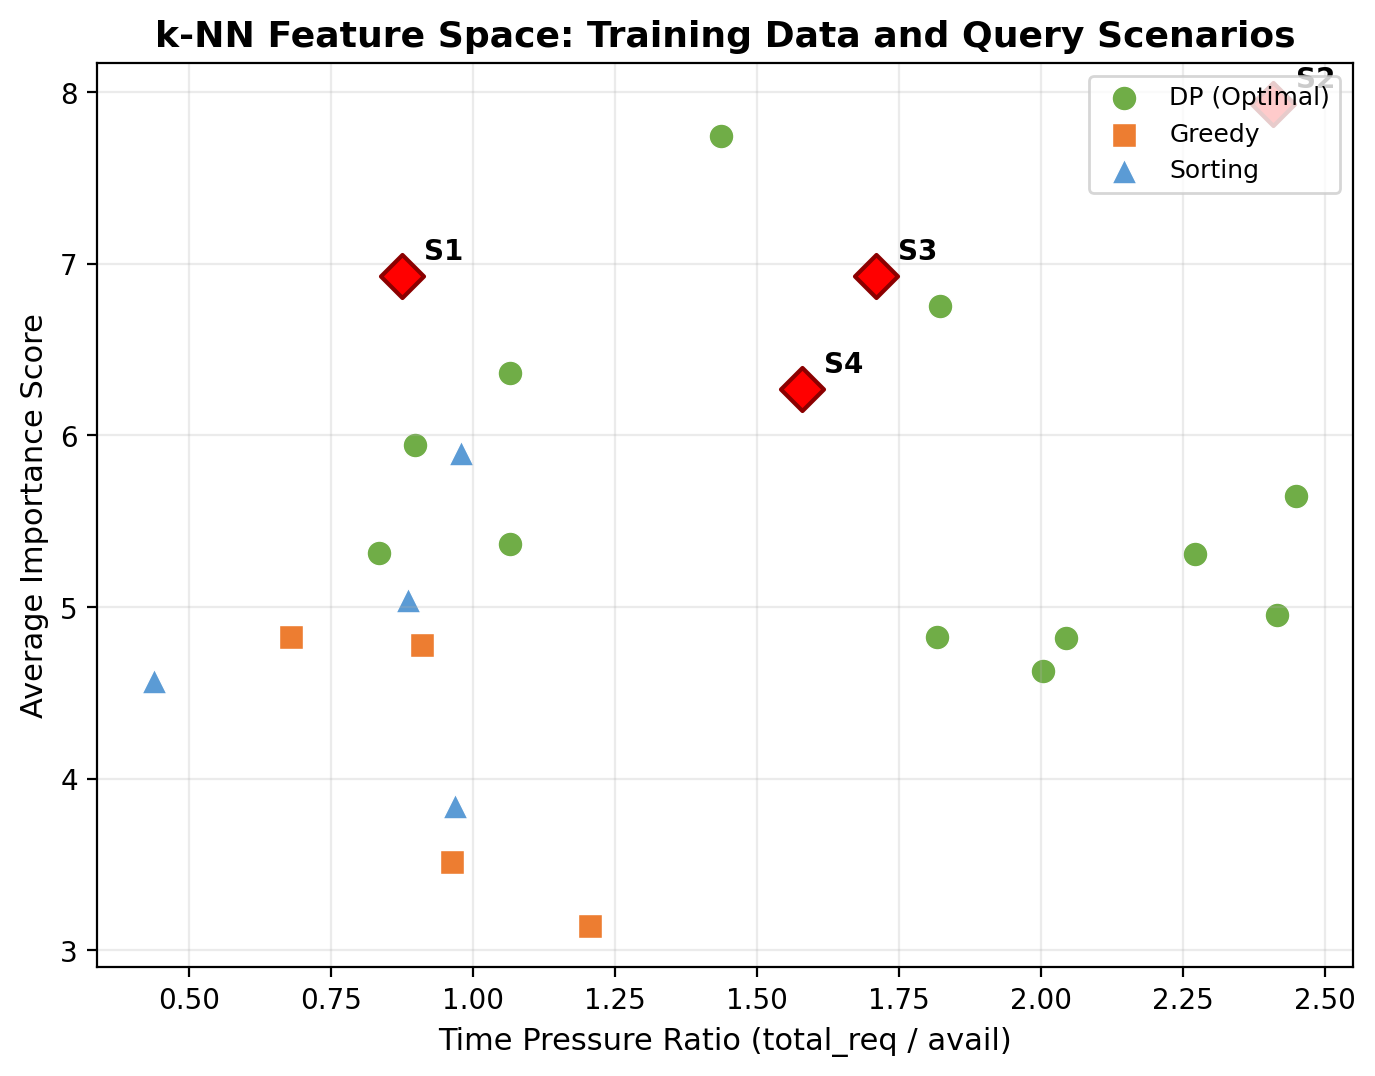
\includegraphics[width=0.92\textwidth]{fig_knn_space.png}
\caption{Training data (circles, squares, triangles) and test
         scenarios (red diamonds) projected onto pressure ratio
         and average importance.}
\label{fig:knn_space}
\end{figure}

\begin{figure}[H]
\centering
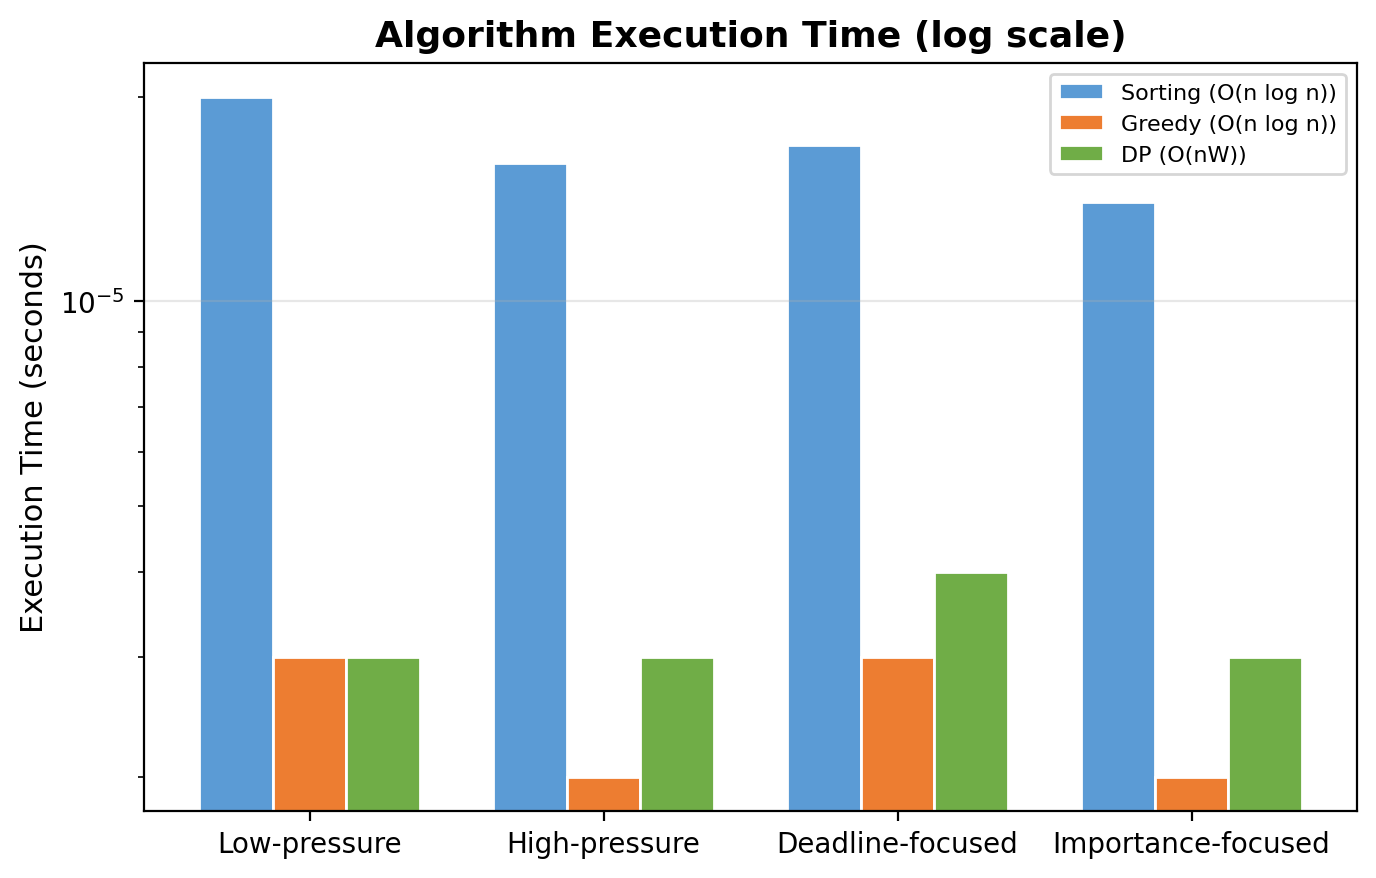
\includegraphics[width=0.92\textwidth]{fig_exec_time.png}
\caption{Execution times on a log scale.  Sorting is consistently
         slowest due to recursive merge overhead.}
\label{fig:exec_time}
\end{figure}


%==============================================================================
\section{Decision Trees as a Natural Contrast}
%==============================================================================

The other half of Option~5 in the group project is the Decision Tree
classifier~\cite{safavian1991survey}.  It is worth examining why we
chose k-NN over this alternative, because the two methods represent
nearly opposite design philosophies.

A Decision Tree works by repeatedly partitioning the feature space.
At each split, the algorithm selects the feature and threshold that
best separate the data according to some impurity measure (typically
Gini impurity or information gain).  The result is a tree-shaped
model where internal nodes represent tests on features and leaf nodes
carry the predicted class.  Once the tree is built, a query is
classified by walking from the root to a leaf, making it extremely
fast at query time --- \(O(\text{tree depth})\), which is typically
\(O(\log N)\) for a balanced tree.

We considered decision trees for StudySmart AI but settled on k-NN
for two reasons.  First, a practical one: our training set has only
16 examples.  A decision tree trained on so few data points is
notoriously prone to overfitting --- it can memorise the exact
feature boundaries of each training sample and fail to generalise.
One could limit the tree depth or set a minimum number of samples per
leaf, but with 16 points there is not much room to prune.  k-NN, by
contrast, makes no attempt to model the distribution at all; it simply
stores the data and defers to the majority vote of the nearest stored
examples.  On a dataset this small, that conservative strategy is
arguably safer.

Second, transparency matters in a teaching context.  A trained decision
tree produces a set of rules (``if pressure ratio \(>\) 1.8 and average
importance \(<\) 6, recommend DP''), which sounds appealing in theory.
In practice, however, a tree built on six features with 16 samples
might end up splitting on features that happen to separate the
training set by chance rather than because they capture a genuine
underlying pattern.  The nearest-neighbour approach is easier to audit:
one can simply look at the three most similar historical scenarios
and verify that the recommendation makes sense~\cite{aha1991instance}.

That said, decision trees have one clear advantage: they are
insensitive to feature scaling.  k-NN requires that we normalise
features (or at least check that the Euclidean distance is not
dominated by one axis), whereas a tree cares only about the ordering
of values along each feature.  This convenience is part of why
decision trees, and in particular their ensemble extensions like
Random Forests, dominate tabular classification in industry
settings~\cite{biau2016random}.  For a 16-sample educational project,
however, the trade-off tilts toward simplicity.


%==============================================================================
\section{Comparison and Reflection}
%==============================================================================

Table~\ref{tab:comparison} summarises how k-NN and Decision Trees
line up across the dimensions that matter for StudySmart AI.

\begin{table}[H]
\centering
\caption{Head-to-head: k-NN versus Decision Tree}
\label{tab:comparison}
\begin{tabular}{@{}p{2.8cm}p{4.2cm}p{4.2cm}@{}}
\toprule
\textbf{Criterion} & \textbf{k-NN} & \textbf{Decision Tree} \\
\midrule
Query efficiency  & \(O(N \log N)\) per query & \(O(\text{tree depth}) \approx O(\log N)\) \\
\addlinespace
Minimum data size & Works with any \(N\) --- lazy learning & Needs enough samples to split reliably \\
\addlinespace
Overfitting risk (small data) & Low --- no explicit model is built & High --- can memorise training points \\
\addlinespace
Implementation    & $\sim$30 lines of C++ & Moderate --- requires split-selection logic \\
\addlinespace
Interpretability  & Transparent --- inspect neighbours directly & Rule-based, but rules may be artefacts \\
\addlinespace
Feature scaling   & Sensitive --- normalisation required & Insensitive to monotonic transforms \\
\addlinespace
Training cost     & \(O(1)\) --- nothing to learn & \(O(Nd \log N)\) --- splits must be evaluated \\
\bottomrule
\end{tabular}
\end{table}

For the current project, k-NN comes out ahead.  The dataset
is simply too small for a decision tree to build meaningful splits:
with only 16 training samples, even a modest tree of depth 2 or 3
risks splitting on quirks of the data rather than genuine patterns.
k-NN sidesteps this by refusing to build a model in the first place,
which on tiny data is a feature, not a bug.

The label-skew problem from Section~3.2 --- every training example
is labelled DP --- affects both methods equally.  A decision tree
would likely collapse to a single leaf predicting DP after examining
the data, which is neither more nor less useful than k-NN's
unanimous vote.  The real limitation is the labelling scheme, not
the classifier.

Decision Trees would start to pull ahead if  If the
scenario library were expanded with dozens of examples that include
cases where Greedy or Sorting actually wins, a shallow decision tree
trained on these richer labels could produce human-readable rules ---
``when pressure is low and importance variance is high, use DP'' ---
that make the recommendation logic explicit.  Ensemble extensions like
Random Forests~\cite{biau2016random} would then be a natural next step,
trading some of that rule-level readability for improved stability.
Within the current scope, though, k-NN does the job with less code
and less risk of overfitting.


%==============================================================================
\begin{thebibliography}{3}

\bibitem{aha1991instance}
D.~W.~Aha, D.~Kibler, and M.~K.~Albert,
``Instance-based learning algorithms,''
\emph{Machine Learning}, vol.~6, pp.~37--66, 1991.
doi: \texttt{10.1007/bf00153759}.

\bibitem{safavian1991survey}
S.~R.~Safavian and D.~A.~Landgrebe,
``A survey of decision tree classifier methodology,''
\emph{IEEE Trans. Syst., Man, Cybern.}, vol.~21, no.~3, pp.~660--674, 1991.
doi: \texttt{10.1109/21.97458}.

\bibitem{biau2016random}
G.~Biau and E.~Scornet,
``A random forest guided tour,''
\emph{Test}, vol.~25, no.~2, pp.~197--227, 2016.
doi: \texttt{10.1007/s11749-016-0481-7}.

\end{thebibliography}

\end{document}
